\documentclass[submit]{harvardml}
\usepackage{common}
\usepackage{float}
\assignment{Homework \#5}
\duedate{April 19, 2026 at 11:59pm}

\usepackage[OT1]{fontenc}
\usepackage[colorlinks,citecolor=blue,urlcolor=blue]{hyperref}
\usepackage{graphicx}
\usepackage{subcaption}
\usepackage{amsmath}
\usepackage{amssymb}
\usepackage{booktabs}
\usepackage{float}
\usepackage{framed}
\usepackage{xcolor}
\usepackage{enumitem}
\graphicspath{{img_output/}}

\newenvironment{solution}{%
    \vspace{2mm}\color{blue}\noindent\textbf{Solution}:\ }
{}

\begin{document}

\begin{center}
{\Large Clustering, PCA, SSL}\\
\end{center}

\subsection*{Overview}
This homework contains four problems:
\begin{enumerate}[leftmargin=*]
    \item SimCLR and contrastive learning.
    \item GANs and the Jensen--Shannon divergence interpretation.
    \item K-means and hierarchical agglomerative clustering on handwritten digits.
    \item PCA on MNIST.
\end{enumerate}
The coding portions are consolidated in \texttt{hw5\_release.ipynb}. The clustering and PCA plots used below are stored in \texttt{img\_output/}.

\subsection*{Resources and Submission Instructions}
Please type your answers after the corresponding problems using this \LaTeX\ template, and start each main problem on a new page.

Please submit the writeup PDF to the Gradescope assignment \texttt{HW5}. Remember to assign pages for each question. \textbf{You must include any plots in your writeup PDF.} Please submit your \LaTeX\ file and code files to the Gradescope assignment \texttt{HW5 - Supplemental}. Your files should be named in the same way as we provide them in the repository, for example \texttt{hw5\_release.tex} and \texttt{hw5\_release.ipynb}.

\begin{problem}[Contrastive Learning]
In this problem we study SimCLR, a self-supervised learning framework that learns visual representations without labels by training a network to identify which data augmentations came from the same image.

This problem mixes short written questions with an implementation scaffold. In the notebook, the SimCLR section is organized in the same order as the written prompt: encoder backbone, projection head, NT-Xent loss, verification, pre-training, and linear evaluation.

\begin{enumerate}[leftmargin=*]
\item \textbf{SimCLR and the NT-Xent loss.}

The SimCLR pipeline works as follows. Given a minibatch of \(N\) images, each image \(x_k\) is augmented twice, producing a positive pair \((\tilde{x}_{2k-1}, \tilde{x}_{2k})\). This yields \(2N\) augmented views total. Each view is passed through an encoder \(f\) and a projection head \(g\) to produce normalized embeddings
\[
\mathbf{z}_i = \frac{g(f(\tilde{x}_i))}{\|g(f(\tilde{x}_i))\|}.
\]
For a positive pair \((i,j)\), the NT-Xent loss is
\[
\ell(i,j) = -\log \frac{\exp(\mathbf{z}_i^\top \mathbf{z}_j / \tau)}{\sum_{k=1,\,k\neq i}^{2N} \exp(\mathbf{z}_i^\top \mathbf{z}_k / \tau)},
\]
where \(\tau > 0\) is a temperature parameter.

\begin{enumerate}[label=(\alph*)]
    \item Show that \(\ell(i,j)\) is equivalent to the cross-entropy loss of a \((2N-1)\)-way classification problem in which the positive partner \(j\) is the correct class and the remaining \(2N-2\) embeddings are negatives.
    \item Consider the softmax weight assigned to a negative sample \(k \neq j\):
    \[
    w_k = \frac{\exp(\mathbf{z}_i^\top \mathbf{z}_k / \tau)}{\sum_{m=1,\,m\neq i}^{2N} \exp(\mathbf{z}_i^\top \mathbf{z}_m / \tau)}.
    \]
    Explain what happens as \(\tau \to 0^+\), what happens as \(\tau \to \infty\), and why an intermediate temperature is preferred in practice.
\end{enumerate}

\item \textbf{Representation collapse and augmentations.}
\begin{enumerate}[label=(\alph*)]
    \item Compute \(\ell(i,j)\) under the collapse solution \(f(x)=\mathbf c\), where \(\mathbf c\) is a constant unit vector and therefore every pairwise similarity is \(1\).
    \item Explain intuitively why the encoder representation \(\mathbf h=f(x)\) is often more useful downstream than the projection-head output \(\mathbf z=g(f(x))\).
    \item Discuss the effect of overly aggressive augmentations and overly weak augmentations on the learned representation.
\end{enumerate}

\item \textbf{Implementing SimCLR components (code).}
In the notebook, implement:
\begin{enumerate}[label=(\alph*)]
    \item a two-layer projection head \(\mathrm{Linear} \to \mathrm{ReLU} \to \mathrm{Linear}\), and
    \item the NT-Xent loss for two batches of projected views.
\end{enumerate}
The intended implementation flow is:
\begin{enumerate}[label=(\roman*)]
    \item \(\ell_2\)-normalize the representations,
    \item concatenate them into a \(2N \times d_z\) matrix,
    \item compute the \(2N \times 2N\) cosine-similarity matrix scaled by \(1/\tau\),
    \item mask self-similarities,
    \item identify the positive-pair index for each view, and
    \item compute cross-entropy loss using the positive index as the target.
\end{enumerate}
The corresponding notebook cells are grouped under the SimCLR headings
\texttt{Projection Head}, \texttt{NT-Xent Loss}, and
\texttt{Run Test Cases}.

\item \textbf{SimCLR training and linear evaluation (code).}
Use the provided training scaffold to:
\begin{enumerate}[label=(\alph*)]
    \item pre-train the encoder and projection head on FashionMNIST without labels,
    \item freeze the encoder and run linear evaluation on top of the learned features, and
    \item compare the resulting linear-evaluation accuracy against a supervised baseline with the same encoder architecture.
\end{enumerate}
In the notebook, these correspond to the sections
\texttt{Data Loading and Augmentations},
\texttt{SimCLR Pre-training},
\texttt{Linear Evaluation}, and
\texttt{Supervised Baseline}.
\end{enumerate}
\end{problem}

\begin{solution}
	\begin{enumerate}
	    \item \begin{enumerate}
	        \item For anchor \(i\), define the score for every other embedding \(k \neq i\) as

\[
s_{ik} = \frac{z_i^\top z_k}{\tau}.
\]

This gives \(2N-1\) possible classes, since among the \(2N\) embeddings we exclude \(i\) itself.
The correct class is the positive pair \(j\), while the remaining \(2N-2\) embeddings are negatives.

Using softmax, the probability of choosing class \(j\) is

\[
p_i(j)
=
\frac{\exp(s_{ij})}
{\sum_{\substack{k=1 \\ k \neq i}}^{2N} \exp(s_{ik})}
=
\frac{\exp\left(z_i^\top z_j/\tau\right)}
{\sum_{\substack{k=1 \\ k \neq i}}^{2N} \exp\left(z_i^\top z_k/\tau\right)}.
\]

The cross-entropy loss for this \((2N-1)\)-way classification problem is

\[
\mathrm{CE}
=
-\log p_i(j).
\]

Substituting the softmax expression gives

\[
\mathrm{CE}
=
-\log
\frac{\exp\left(z_i^\top z_j/\tau\right)}
{\sum_{\substack{k=1 \\ k \neq i}}^{2N}
\exp\left(z_i^\top z_k/\tau\right)}.
\]

This is exactly

\[
\ell(i,j)
=
-\log
\frac{\exp\left(z_i^\top z_j/\tau\right)}
{\sum_{\substack{k=1 \\ k \neq i}}^{2N}
\exp\left(z_i^\top z_k/\tau\right)}.
\]

Therefore, the NT-Xent loss is exactly the cross-entropy loss of a \((2N-1)\)-class classification problem where the model must identify the positive partner \(j\) of anchor \(i\) among all other embeddings.
\item For a negative sample \(k \neq j\), the softmax weight is

\[
w_k
=
\frac{\exp\left(z_i^\top z_k / \tau\right)}
{\sum_{\substack{m=1 \\ m \neq i}}^{2N}
\exp\left(z_i^\top z_m / \tau\right)}.
\]

As \(\tau \to 0^{+}\), the quantity \(\frac{z_i^\top z_k}{\tau}\) becomes very large for the sample with the
largest similarity to \(z_i\), and much smaller for all others. That's why the softmax becomes nearly
a hard maximum, meaning almost all probability mass is assigned to the most similar sample

If the most similar sample is a hard negative, it receives nearly all the weight, while the rest receive
almost zero weight. This creates very steep gradients and makes training unstable.

As \(\tau \to \infty\), we have

\[
\frac{z_i^\top z_k}{\tau} \to 0
\]

for all \(k\), so

\[
\exp\left(z_i^\top z_k / \tau\right) \approx 1.
\]

Thus all samples receive nearly equal weight:

\[
w_k \approx \frac{1}{2N-1}.
\]


An intermediate temperature is preferred because it balances these two edge cases in the sense that it gives higher
weight to informative hard negatives without making the optimization too unstable. This provides
useful gradients while maintaining stable training.
	    \end{enumerate}
        \item \begin{enumerate}
            \item Under collapse, every normalized representation is the same unit vector \(c\), so for all
\(m \neq i\),

\[
z_i^\top z_m = 1.
\]

Hence

\[
\ell(i,j)
=
-\log
\frac{\exp(1/\tau)}
{\sum_{\substack{k=1\\k\neq i}}^{2N}\exp(1/\tau)}.
\]

There are \(2N-1\) terms in the denominator, all equal to \(\exp(1/\tau)\), so

\[
\ell(i,j)
=
-\log
\frac{\exp(1/\tau)}
{(2N-1)\exp(1/\tau)}
=
-\log\left(\frac{1}{2N-1}\right).
\]

Therefore,

\[
\boxed{\ell(i,j)=\log(2N-1).}
\]
            \item The encoder output \(h=f(x)\) is usually more useful downstream because it is the
representation that is meant to capture the semantic content of the image. The projection head \(g\)
is trained specifically to help optimize the contrastive objective, so \(z=g(f(x))\) may discard
information that is useful for transfer but unnecessary for the pretraining loss. Thus \(h\) tends to
be more of a general representation, while \(z\) is more specialized to SimCLR training.
            \item If augmentations are too aggressive, two views of the same image may no longer preserve
the same semantics . Then the model is forced to pull together representations that should not
really match, which can hurt the learned features.

If augmentations are too weak, the two views are nearly identical, so the task becomes too easy.
The model can solve it using low-level cues instead of learning complex semantic features.

An intermediate augmentation strength is preferred because it preserves the underlying identity of the
image while still forcing the model to become invariant to nuisance changes.
        \end{enumerate}
\item   SimCLR Pre training Loss

    \centering
    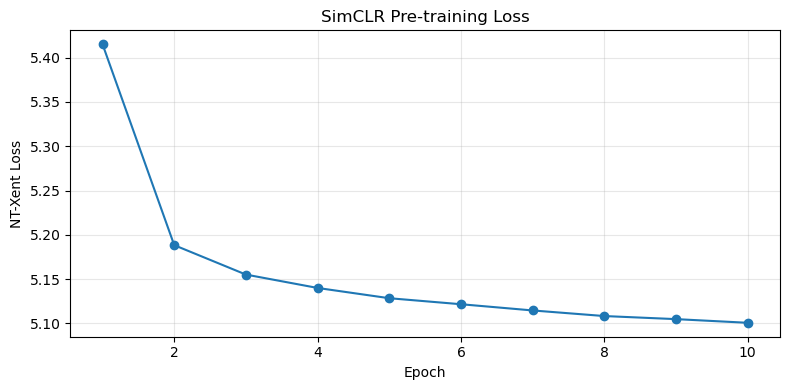
\includegraphics[width=0.5\linewidth]{simCLRLoss.png}
    \item SimCLR vs Supervised 
    
    \centering
    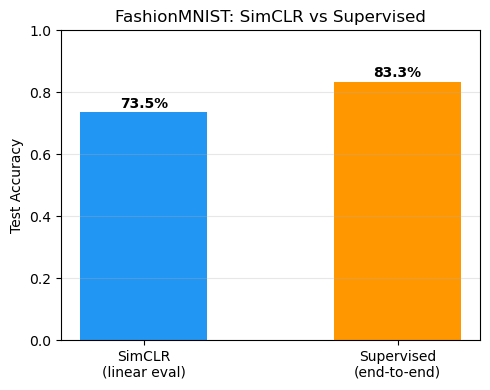
\includegraphics[width=0.5\linewidth]{Comparison.png}
		\end{enumerate}
\end{solution}

\newpage

\begin{problem}[GANs]
Consider the original minimax GAN objective
\[
\min_G \max_D V(D,G) = \mathbb E_{x\sim p_{\mathrm{data}}}[\log D(x)] + \mathbb E_{z\sim p_z}[\log(1-D(G(z)))] .
\]
Let \(p_g\) denote the distribution induced by \(x = G(z)\).

This problem has both a written component and a coding component.

\begin{itemize}[leftmargin=*]
    \item \textbf{Written work:} derive the optimal discriminator, rewrite the GAN objective in terms of the Jensen--Shannon divergence, and explain the resulting training objectives in words and equations.
    \item \textbf{Code work:} implement the practical GAN training loop in the notebook by defining the generator and discriminator, implementing the discriminator and generator losses, and alternating the two updates during training.
\end{itemize}

The GAN notebook section is deliberately split into small cells so that the mathematical objectives and the alternating training logic are easy to match to the code. The intended order is data setup, model definitions, loss definitions, one-epoch training logic, and then the multi-epoch training loop.

\begin{enumerate}[leftmargin=*]
    \item \textbf{Interpreting GANs as Jensen--Shannon divergence (written).}
    Assume \(G\) is fixed.
    \begin{enumerate}[label=(\alph*)]
        \item Derive the optimal discriminator \(D^*(x)\) in terms of \(p_{\mathrm{data}}(x)\) and \(p_g(x)\).
        \item Substitute \(D^*(x)\) back into the GAN objective and show that the result can be written as a constant plus a Jensen--Shannon divergence term.
        \item Explain, in words, what this means for what the generator is trying to do.
    \end{enumerate}
    \item \textbf{From derivation to training algorithm (written).}
    \begin{enumerate}[label=(\alph*)]
        \item Write the discriminator objective.
        \item Write the generator objective.
        \item Describe the alternating training loop used in practice.
    \end{enumerate}
    \item \textbf{GAN implementation (code).}
    In the notebook, complete the practical GAN scaffold by:
    \begin{enumerate}[label=(\alph*)]
        \item defining the generator and discriminator networks,
        \item implementing the discriminator loss on real and fake batches,
        \item implementing the generator loss,
        \item writing the alternating update logic for one epoch of training, and
        \item training for multiple epochs and visualizing generated samples.
    \end{enumerate}
    In \texttt{hw5\_release.ipynb}, these correspond to the GAN section cells for model setup, loss definitions, \texttt{train\_one\_epoch}, and the final training loop.
\end{enumerate}
\end{problem}

\begin{solution}
	\begin{enumerate}
	    \item \begin{enumerate}
	        \item For fixed \(G\), the objective is

\[
V(D,G)
=
\mathbb{E}_{x \sim p_{\mathrm{data}}}[\log D(x)]
+
\mathbb{E}_{x \sim p_g}[\log(1-D(x))].
\]

Writing this as an integral,

\[
V(D,G)
=
\int p_{\mathrm{data}}(x)\log D(x)\,dx
+
\int p_g(x)\log(1-D(x))\,dx.
\]

Since this is pointwise in \(x\), for each fixed \(x\) we maximize

\[
p_{\mathrm{data}}(x)\log D(x) + p_g(x)\log(1-D(x)).
\]

Let

\[
a = p_{\mathrm{data}}(x), \qquad b = p_g(x).
\]

Then we maximize

\[
a \log D(x) + b \log(1-D(x)).
\]

Differentiate :

\[
\frac{a}{D(x)} - \frac{b}{1-D(x)} = 0.
\]

So

\[
a(1-D(x)) = bD(x)
\]

\[
a = (a+b)D(x).
\]

Hence

\[
\boxed{
D^*(x)=\frac{p_{\mathrm{data}}(x)}{p_{\mathrm{data}}(x)+p_g(x)}
}.
\]
            \item Substitute \(D^*(x)\) 

\[
V(D^*,G)
=
\int p_{\mathrm{data}}(x)\log \frac{p_{\mathrm{data}}(x)}{p_{\mathrm{data}}(x)+p_g(x)}\,dx
+
\int p_g(x)\log \frac{p_g(x)}{p_{\mathrm{data}}(x)+p_g(x)}\,dx.
\]

Define

\[
m(x)=\frac{1}{2}\bigl(p_{\mathrm{data}}(x)+p_g(x)\bigr).
\]

Then

\[
p_{\mathrm{data}}(x)+p_g(x)=2m(x),
\]

so

\[
V(D^*,G)
=
\int p_{\mathrm{data}}(x)\log \frac{p_{\mathrm{data}}(x)}{2m(x)}\,dx
+
\int p_g(x)\log \frac{p_g(x)}{2m(x)}\,dx.
\]

Split

\[
V(D^*,G)
=
\int p_{\mathrm{data}}(x)\log \frac{p_{\mathrm{data}}(x)}{m(x)}\,dx
+
\int p_g(x)\log \frac{p_g(x)}{m(x)}\,dx
-2\log 2.
\]

Thus

\[
V(D^*,G)
=
\mathrm{KL}(p_{\mathrm{data}} \,\|\, m)
+
\mathrm{KL}(p_g \,\|\, m)
-2\log 2.
\]

Using

\[
\mathrm{JS}(p_{\mathrm{data}} \,\|\, p_g)
=
\frac{1}{2}\mathrm{KL}(p_{\mathrm{data}} \,\|\, m)
+
\frac{1}{2}\mathrm{KL}(p_g \,\|\, m),
\]

we get

\[
\boxed{
V(D^*,G)
=
- \log 4
+
2\,\mathrm{JS}(p_{\mathrm{data}} \,\|\, p_g)
}.
\]
            \item This means that once the discriminator is optimal, training the generator is equivalent to minimizing

\[
\mathrm{JS}(p_{\mathrm{data}} \,\|\, p_g).
\]

So the generator is trying to make the model distribution \(p_g\) match the true data distribution \(p_{\mathrm{data}}\). The best case is when

\[
p_g = p_{\mathrm{data}},
\]

because then

\[
\mathrm{JS}(p_{\mathrm{data}} \,\|\, p_g)=0
\]

and

\[
V(D^*,G) = -\log 4.
\]

The generator is trying to produce samples so realistic that the discriminator cannot differentiate what is real from what is fake, in both cases 

\[
D^*(x)=\frac{1}{2}
\]

everywhere.
	    \end{enumerate}
        \item \begin{enumerate}
            \item The discriminator is trained to maximize

\[
\mathcal{L}_D
=
\mathbb{E}_{x \sim p_{\mathrm{data}}}[\log D(x)]
+
\mathbb{E}_{z \sim p_z}[\log(1-D(G(z)))].
\]

If we take it in minimization form we minimize

\[
J_D
=
-\mathcal{L}_D
=
-\mathbb{E}_{x \sim p_{\mathrm{data}}}[\log D(x)]
-
\mathbb{E}_{z \sim p_z}[\log(1-D(G(z)))].
\]

            \item In the original  formulation, the generator minimizes

\[
\mathcal{L}_G^{\mathrm{minimax}}
=
\mathbb{E}_{z \sim p_z}[\log(1-D(G(z)))].
\]

But we use generator loss

\[
\mathcal{L}_G
=
-\mathbb{E}_{z \sim p_z}[\log D(G(z))],
\]

since it gives stronger gradients when the discriminator is sure.
            \item training alternates between the two updates:

\[
\text{(1) Update } D \text{ with } G \text{ fixed,}
\]
using one minibatch of real samples \(x \sim p_{\mathrm{data}}\) and one minibatch of fake samples
\(G(z)\) with \(z \sim p_z\).

Then

\[
\text{(2) Update } G \text{ with } D \text{ fixed,}
\]
by sampling latent vectors \(z \sim p_z\), generating fake samples \(G(z)\), and taking the gradient
on the  loss.

So each iteration is:

\[
\text{sample real data} \;\to\; \text{sample noise} \;\to\; \text{update } D \;\to\; \text{sample noise again} \;\to\; \text{update } G.
\]

The discriminator learns to distinguish real from fake, while the generator learns to make fake
samples look real enough to "deceive" the discriminator.
        \end{enumerate}
    \item 
    Full training run and evalutaion
    
    \centering
    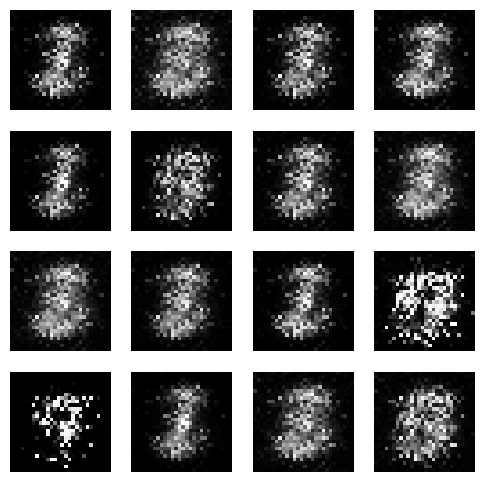
\includegraphics[width=0.25\linewidth]{clusters.png}
	\end{enumerate}

\end{solution}

\newpage

\begin{problem}[K-Means and HAC]
For this problem, K-means and hierarchical agglomerative clustering are implemented from scratch and applied to handwritten-digit data.

Your job is to implement K-means and HAC on MNIST and test whether these relatively simple algorithms can cluster similar-looking images together. The clustering section of the notebook is organized by subproblem number so that each saved figure can be traced back to the corresponding written prompt.

\begin{enumerate}[leftmargin=*]
    \item The code loads the images into two arrays: \texttt{large\_dataset}, a \(5000 \times 784\) array used for K-means, and \texttt{small\_dataset}, a \(300 \times 784\) array used for HAC. A companion array \texttt{small\_dataset\_labels} is used only for the confusion-matrix comparison. In your code, use the \(\ell_2\) norm (Euclidean distance) as the distance metric.
    \item Starting from a random initialization with \(K=10\), plot the K-means objective function as a function of iteration and verify that it never increases.
    \item For \(K=10\) and three random restarts, display the mean image for each cluster. Present the \(30\) total images in a single plot.
    \item Repeat the previous part after standardizing each pixel to have mean \(0\) and variance \(1\), dividing by \(1\) for any zero-variance pixels. Compare the resulting centroids to the unstandardized case.
    \item Implement HAC for max, min, and centroid linkage. Fit each method to the small dataset and show the mean image for each cluster when there are exactly \(10\) clusters. Comment on crispness and explain why HAC only needs one run.
    \item For each HAC linkage and for one K-means run, plot the number of images in each cluster at the stage where there are \(10\) clusters. Explain what these plots say about max-linkage versus min-linkage behavior.
    \item Using the K-means and HAC assignments on the small dataset, plot the pairwise confusion matrices between the clustering methods. Identify which HAC variant is closest to K-means and explain why.
    \item Discuss whether clustering is a good strategy for digit identification, whether clusters should be expected to match true labels, and what kinds of bad or adversarial data are especially problematic for clustering methods.
\end{enumerate}
\end{problem}

\begin{solution}
	\begin{enumerate}
	    \item 
        Verified: objective never increases
        
	 
	    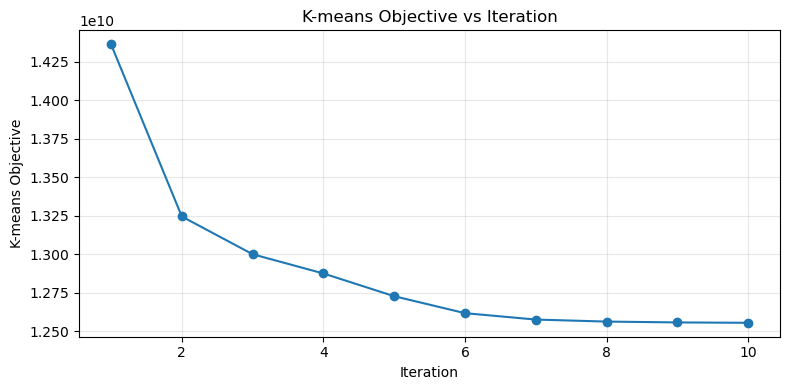
\includegraphics[width=0.5\linewidth]{K-meansObjective.png}
        
        \item 

        Mean Images from Raw Pixels
        
        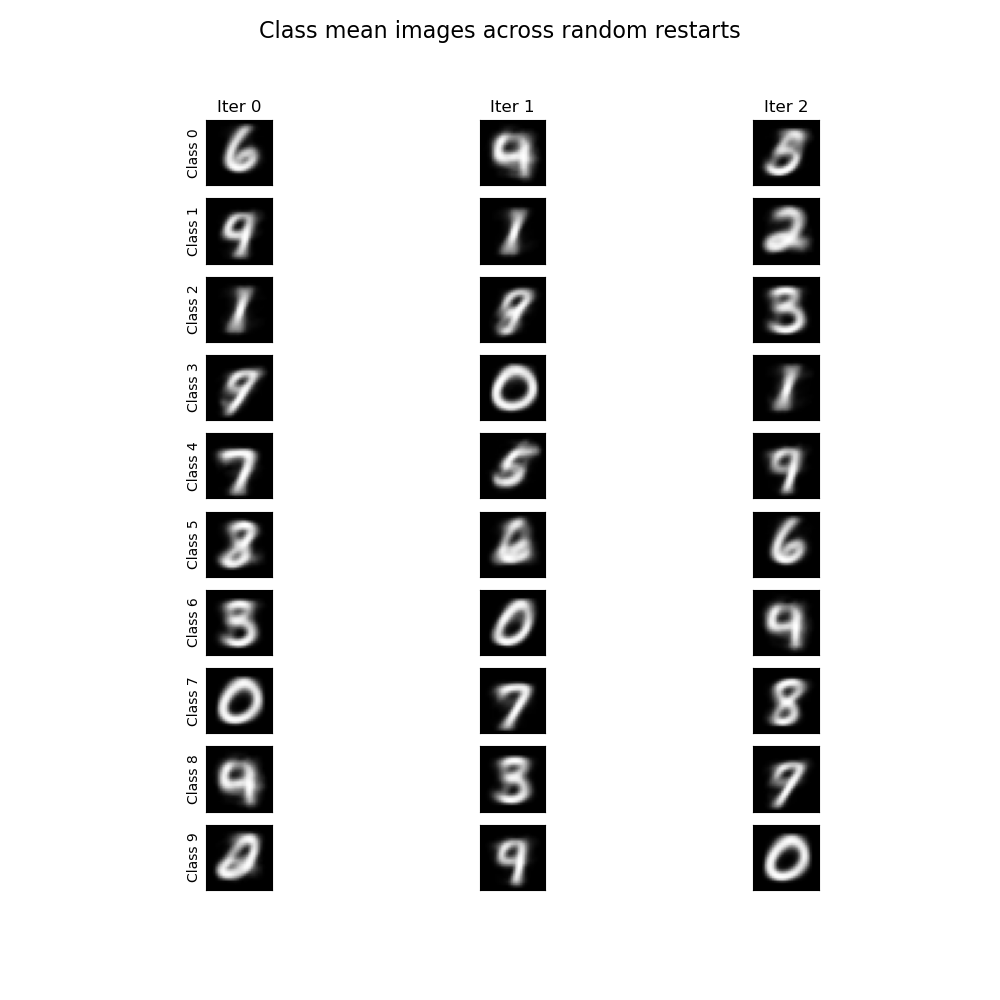
\includegraphics[width=0.5\linewidth]{p2.2.png}

        \item 
        
        Mean Images after Standardization
        
        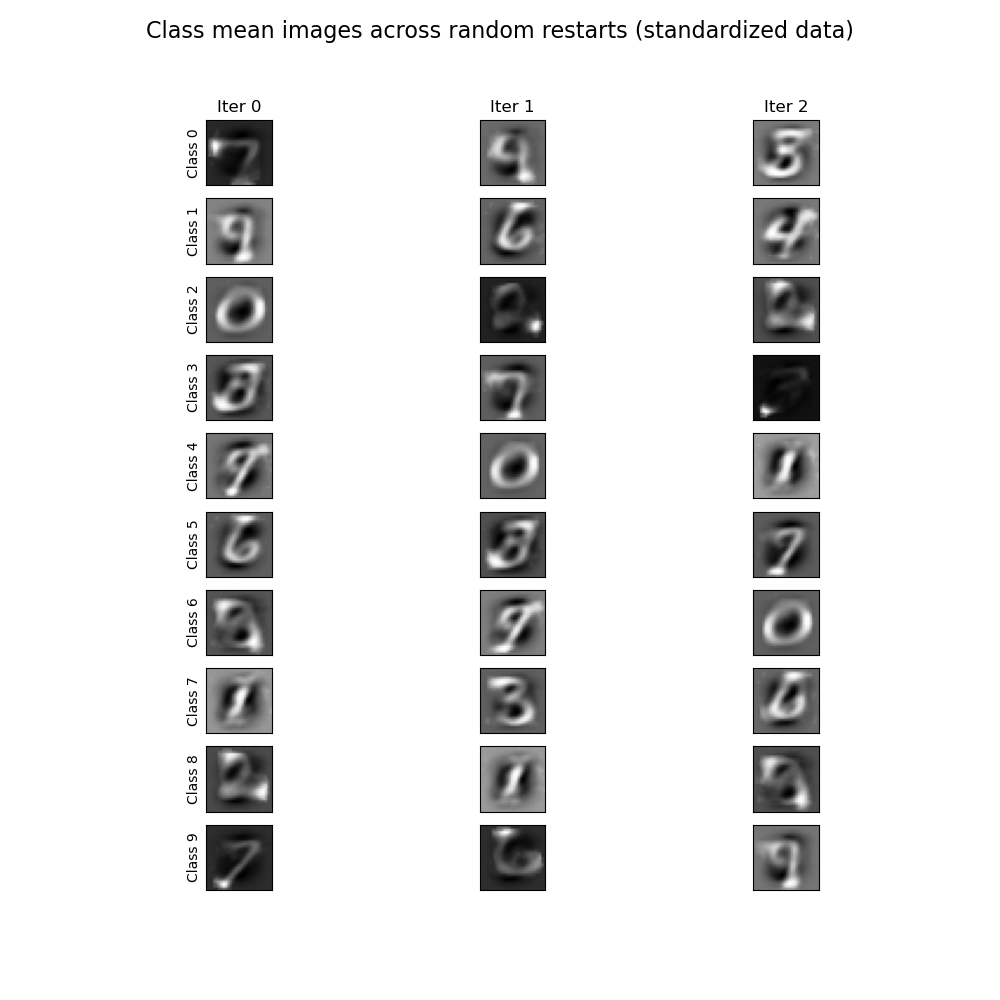
\includegraphics[width=0.5\linewidth]{p2.3.png}

        \item 

        HAC Mean Images
        
        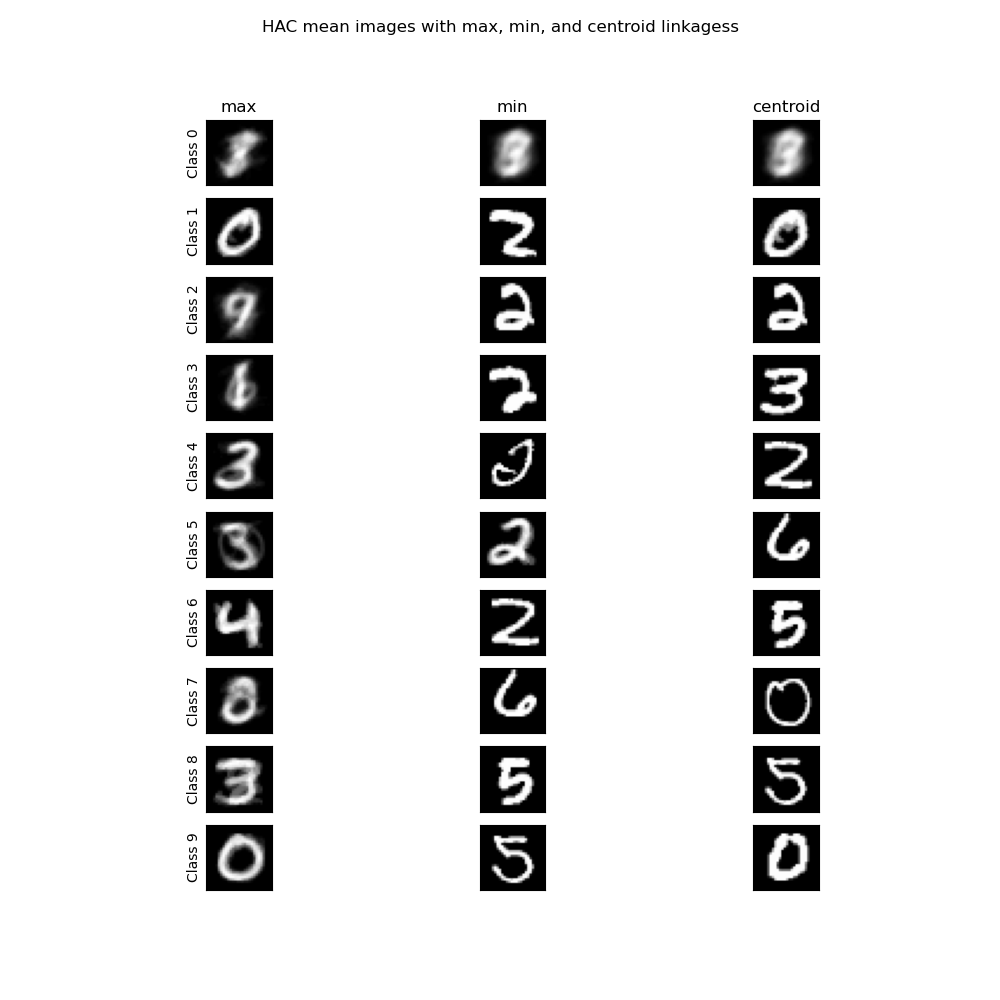
\includegraphics[width=0.5\linewidth]{p2.4.png}

        \item 

        HAC Mean Images
        
        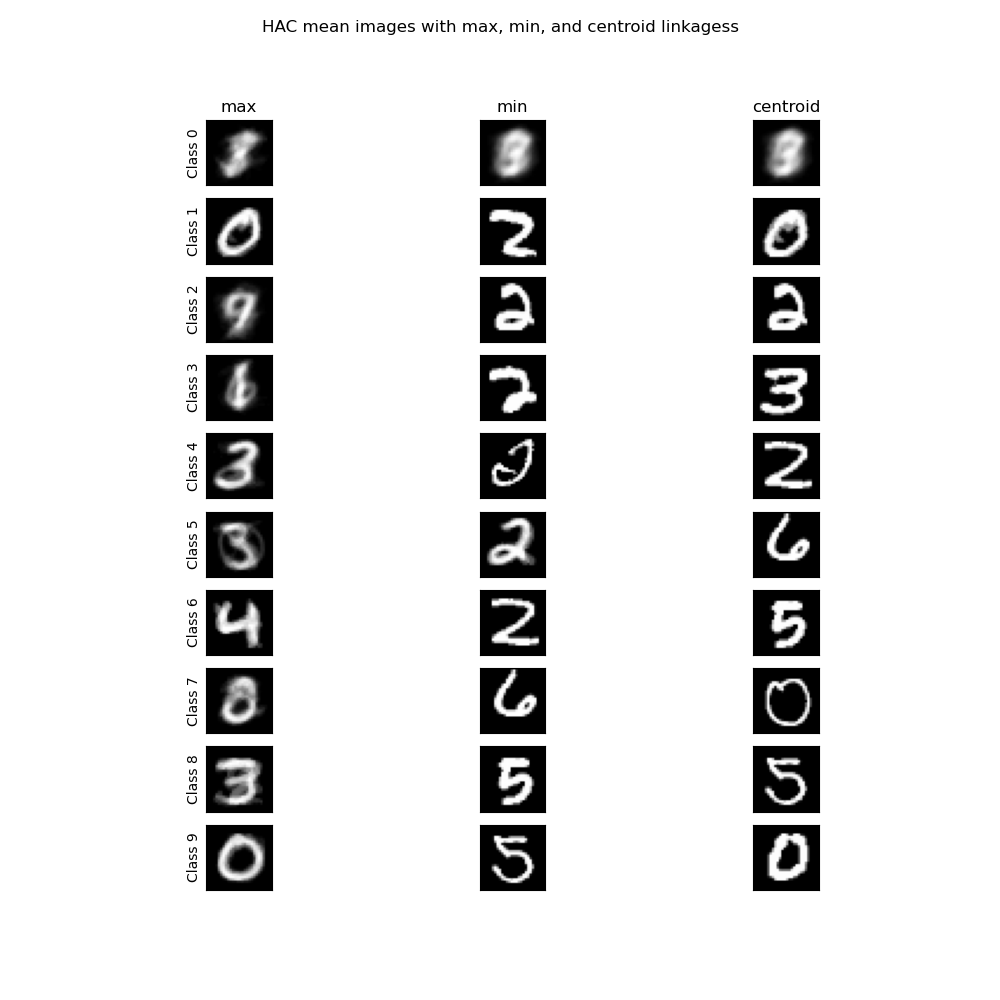
\includegraphics[width=0.5\linewidth]{p2.4.png}

        \item 

        Cluster-Size Plots

        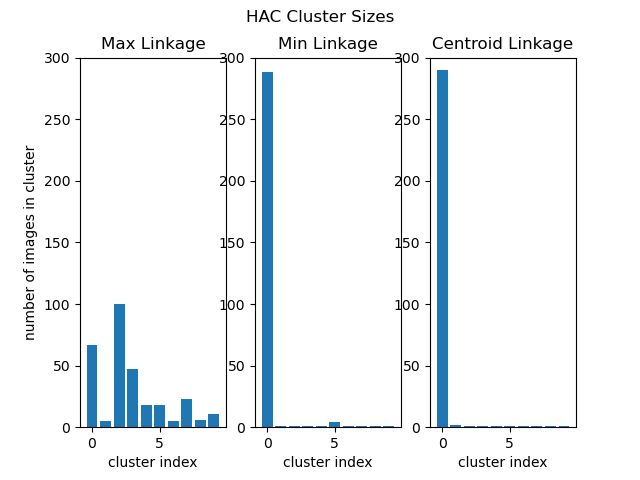
\includegraphics[width=0.5\linewidth]{p2.5a.png}

        \item 

        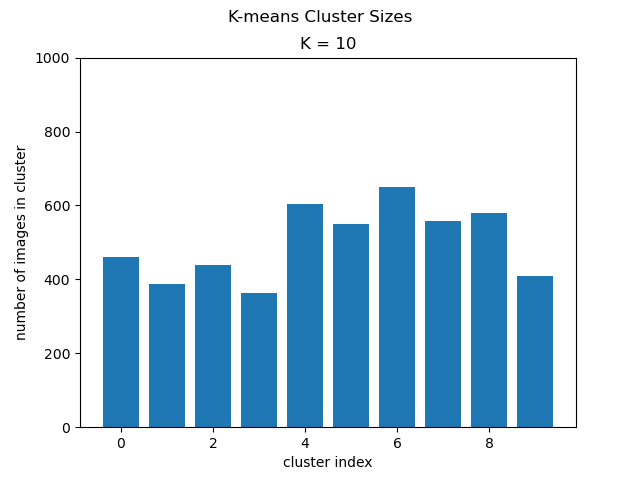
\includegraphics[width=0.5\linewidth]{p2.5b.png}

        \item 

        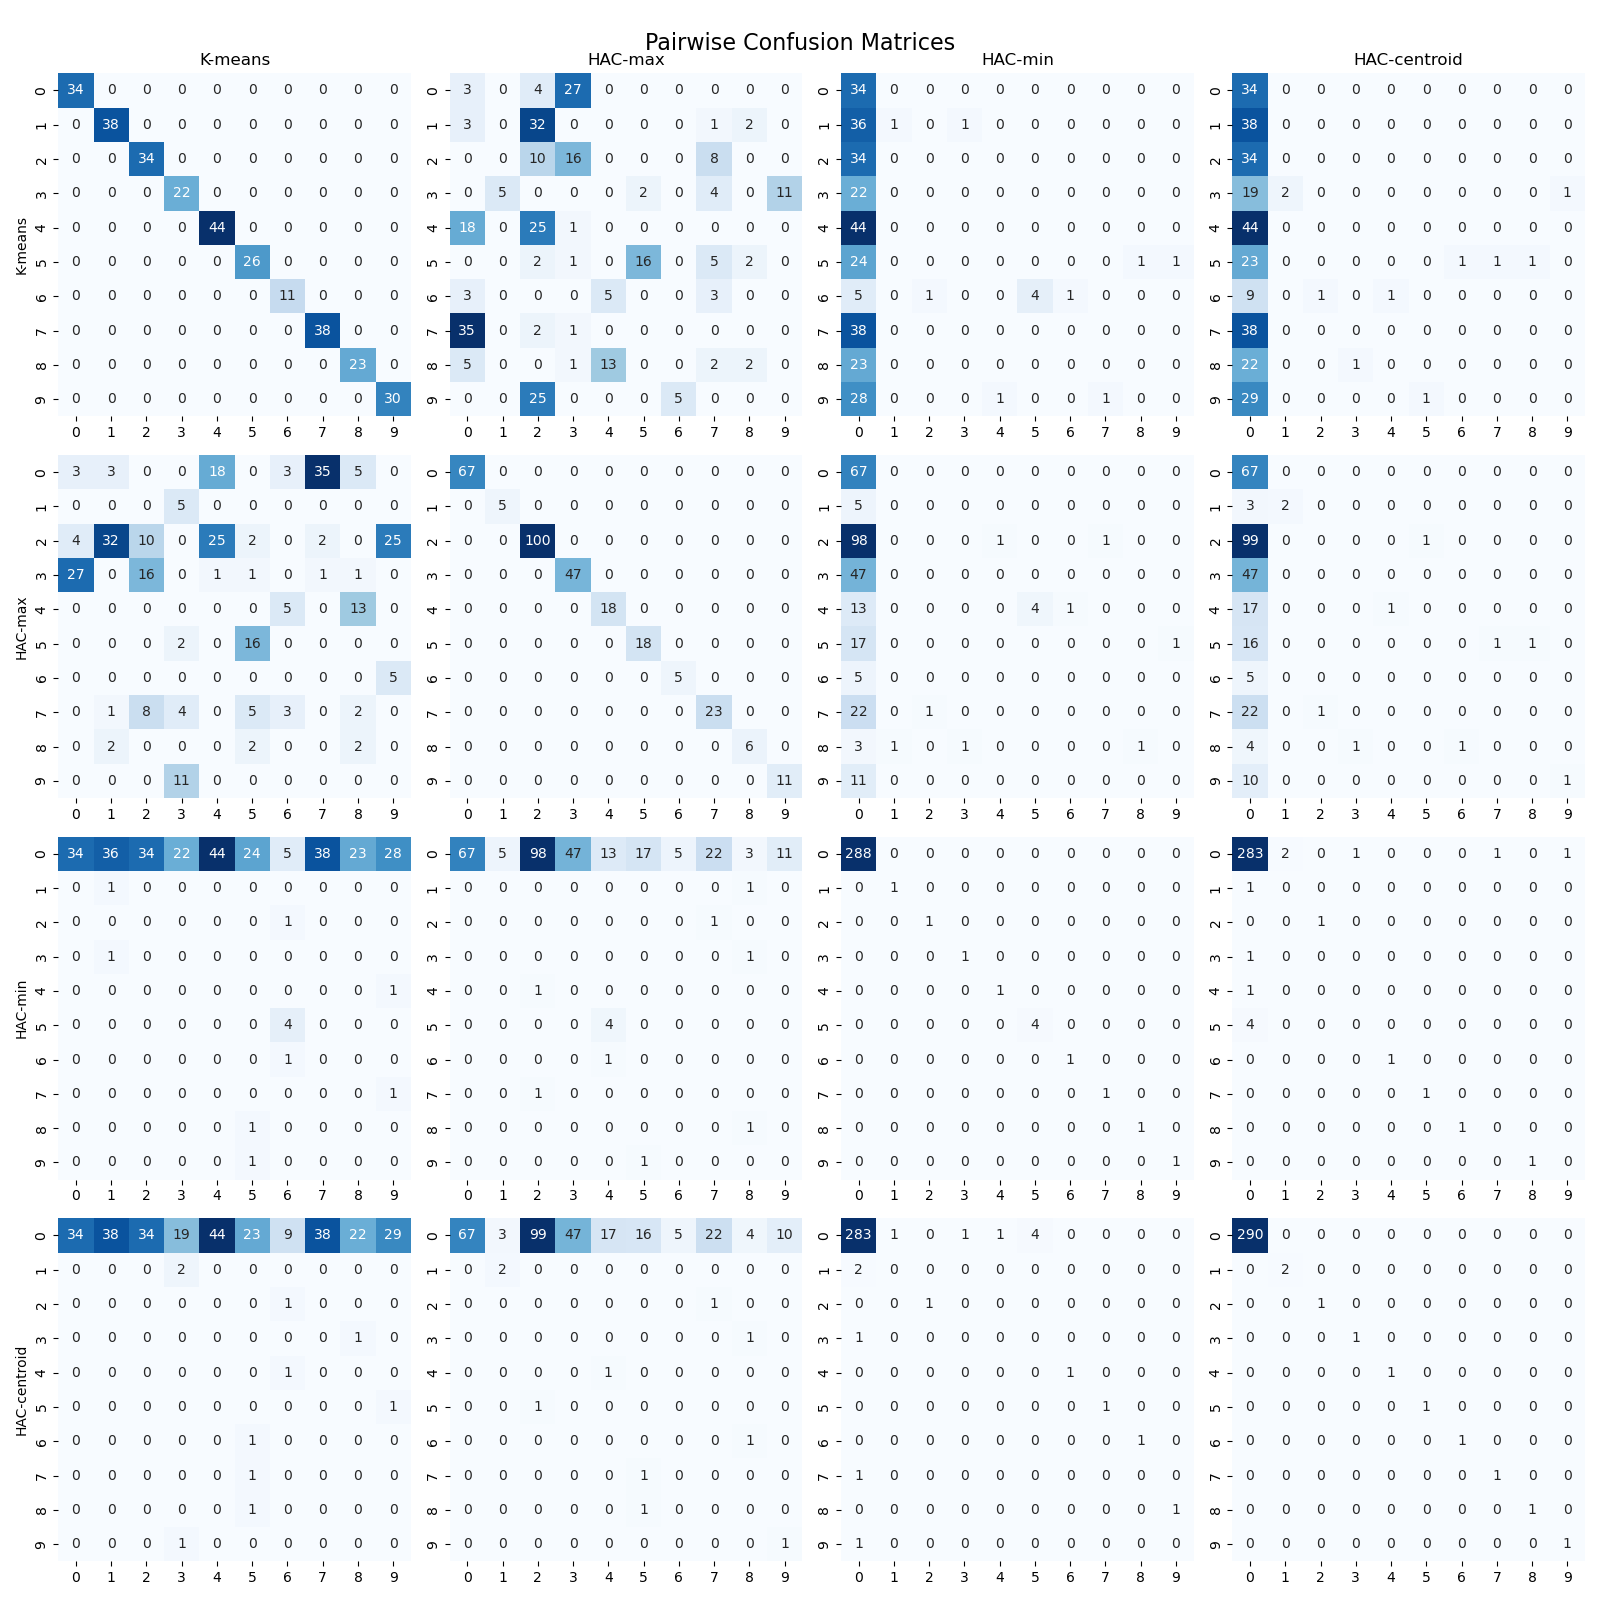
\includegraphics[width=0.5\linewidth]{p2_confusion.png}

         
        
		\end{enumerate}
\end{solution}

\newpage

\begin{problem}[PCA]

  For this problem you will implement PCA from scratch on the first 6000 images of the MNIST dataset. Your job is to apply PCA on MNIST and discuss what kind of structure is found. Implement your solution in \texttt{hw5\_release.ipynb} and attach the final plots below. \\

  \noindent {\bfseries Do not use third-party PCA implementations (for example, {\normalfont \texttt{scikit-learn}}).}
  \begin{enumerate}

    \item Compute the PCA. Plot the eigenvalues corresponding to the most
    significant 500 components in order from most significant to
    least. Make another plot that describes the cumulative proportion of
    variance explained by the first $k$ most significant components for
    values of $k$ from 1 through 500.  How much variance is explained by
    the first 500 components?  Describe how the cumulative proportion of
    variance explained changes with $k$.  Include this plot below.

    \item Plot the mean image of the dataset and plot an image
    corresponding to each of the first 10 principle components.  How do
    the principle component images compare to the cluster centers from
    K-means? Discuss any similarities and differences.  Include these
    two plots below.
    
    \textit{Reminder: Center the data before performing PCA.}

    \item Compute the reconstruction error on the dataset using the first 10 principal components. Then compute the reconstruction error when the reconstruction for each point is just the mean
    image of the dataset. How do these errors compare to
    the final objective loss achieved by using K-means on the dataset?
    Discuss any similarities and differences.

    For consistency in grading, define the error function as the squared L2
    norm of the difference between the true data and the reconstruction, averaged over all data points.
  
    \item Suppose you took the original matrix of principle components
    that you found $V$ and multiplied it on the right side by some rotation matrix $R$ (i.e., you considered the matrix $VR$).
    Would that change the quality of the reconstruction error in the
    last problem?  The interpretation of the components?  Why or why
    not?

  \end{enumerate}
\end{problem}

\begin{solution}
	\begin{enumerate}
	    \item
        The first 500 components capture nearly all the variance. The cumulative curve rises steeply through 50 percent, then flattens past k200.
        Indicating MNIST digits occupy a low-dimensional subspace
        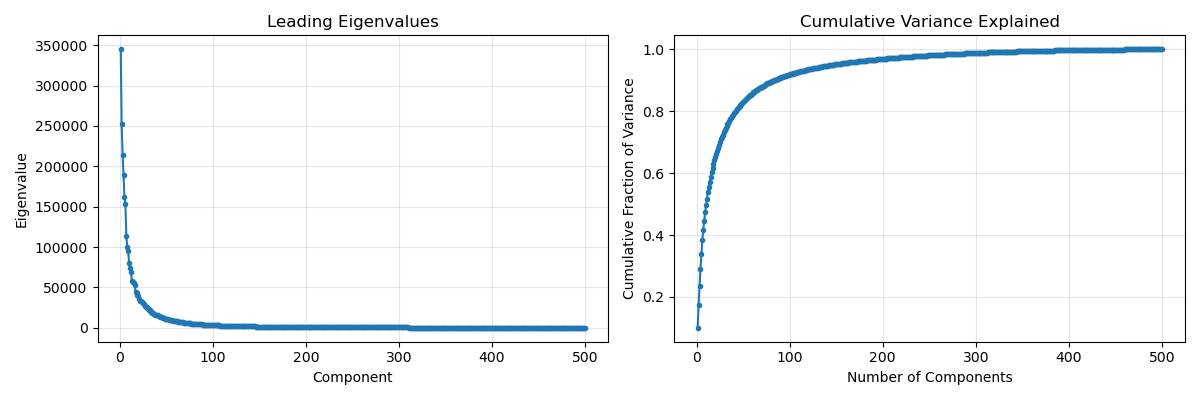
\includegraphics[width=0.75\linewidth]{pca_eigenvalues.png}
        \item 
        K-means cluster centers are interpretable averages — each looks like a blurry but recognizable digit (0, 1, 3, 7, etc.) because K-means partitions the data and computes the mean within each partition. They represent "typical" instances of digit groups.

Principal components look nothing like actual digits. They have both positive and negative values (light and dark contrast regions) and resemble oscillatory patterns or "eigenfaces"-style masks. This is because PCs are orthogonal directions of maximum variance, not cluster prototypes. They capture global modes of variation ( PC1 distinguishes digits with a central loop like 0 from those without; later PCs capture increasingly fine-grained stroke variations).

        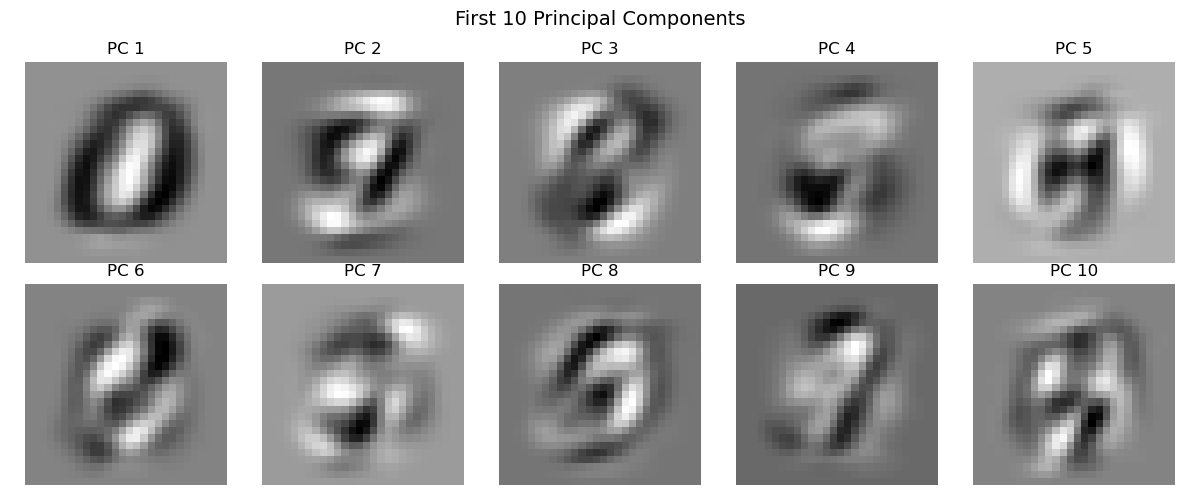
\includegraphics[width=0.75\linewidth]{pca_components.png}

        \item he mean-only reconstruction error (~3.4M per point) is the largest since it uses a single global prototype for all images. K-means (K=10) reduces this to ~2.5M per point by assigning each image to one of 10 cluster centroids, capturing coarse digit-level structure. Top-10 PCA achieves the lowest error (~1.7M per point) despite also using 10 "dimensions," because it reconstructs each image as a unique linear combination of 10 continuous basis vectors rather than snapping to one of 10 fixed prototypes. Both methods exploit the same underlying low-dimensional structure in the data, but PCA's per-image continuous coefficients give it strictly more representational flexibility than K-means' discrete assignments, explaining why PCA's reconstruction error is lower.

        \item Rotating the principal components by an orthogonal matrix $R$ does not change the reconstruction error because VR spans the same subspace as V, and the orthogonality of $ R$ preserves all norms ($R^T R = I$), so projections onto the subspace remain identical. However, it does change the interpretation of individual components: the original PCs are uniquely defined (up to sign) as successive directions of maximum variance, whereas the rotated components mix these directions, even though collectively they represent the same subspace equally well.
	\end{enumerate}
\end{solution}

\end{document}
